\documentclass[a4paper,fleql]{cas-sc}
\usepackage[authoryear,longnamesfirst]{natbib}
\usepackage{amsmath}
\usepackage{amssymb}
\DeclareMathAlphabet{\mathcal}{OMS}{cmsy}{m}{n}
\DeclareMathOperator*{\argmax}{arg\,max}
\usepackage{booktabs}
\usepackage{needspace}
\usepackage{graphicx}
\usepackage{algorithm}
\usepackage{algpseudocode}
\usepackage{multirow}
\usepackage{placeins}
\usepackage{float}
\usepackage{caption}
\usepackage{threeparttable}
\usepackage{tcolorbox}
\usepackage{xspace}

\makeatletter
\def\fps@figure{htbp}
\makeatother

%% Section numbers appear as S1, S2, ...
\renewcommand{\thesection}{S\arabic{section}}
\renewcommand{\thesubsection}{S\arabic{section}.\arabic{subsection}}
\renewcommand{\thesubsubsection}{S\arabic{section}.\arabic{subsection}.\arabic{subsubsection}}

%% Table/Figure prefixes: keep original numbering to preserve cross-refs from main
%% (tab:data, tab:efficiency_app, etc. are referenced by label, not number)

\begin{document}
\let\WriteBookmarks\relax

\title[mode=title]{NexRoute: Supplementary Material}

\author[1]{Junyoung Kong}
\author[1]{Youngguk Ha}

\affiliation[1]{%
    organization={Department of Computer Science and Engineering, Konkuk University},
    addressline={120 Neungdong-ro},
    city={Gwangjin-gu, Seoul},
    postcode={05029},
    country={Republic of Korea}
}

\maketitle

\noindent This document provides supplementary material for the main paper
``NexRoute: A Dual-Axis Nexus Routing Framework for Adaptive Expert Selection
in Cross-Domain Large Language Models.'' Sections are numbered S1--S8 and
correspond to the Supplementary Material references in the main text.

\tableofcontents

\clearpage

%%==============================================================================
\section{Dataset Composition and Quality Control}
\label{supp:dataset}
%%==============================================================================

\vspace{6pt plus 4pt minus 3pt}
\begin{center}
\begingroup
\captionof{table}{Domain corpus statistics. For single-domain partitions,
raw counts denote original MMLU subset sizes and final counts reflect items
retained after quality filtering.
The \texttt{CROSS} partition contains no MCQ-format items as it is
synthesized directly in open-ended instruction-answer format; consequently,
raw and final counts are identical by construction.}
\label{tab:data}
\begin{tabular}{llrr}
\toprule
\textbf{Domain} & \textbf{Representative MMLU Subjects} & \textbf{Raw} & \textbf{Final} \\
\midrule
LAW   & jurisprudence, international\_law, professional\_law  & 5{,}000 & 4{,}968 \\
MED   & clinical\_knowledge, medical\_genetics, nutrition      & 3{,}860 & 3{,}854 \\
SOC   & sociology, econometrics, security\_studies             & 3{,}399 & 2{,}193 \\
STEM  & college\_physics, abstract\_algebra, astronomy         & 3{,}456 & 3{,}408 \\
CROSS & Interdisciplinary synthesized domain-pairs             & 1{,}321 & 1{,}321 \\
\midrule
\textbf{Total} & & \textbf{17{,}036} & \textbf{15{,}744} \\
\bottomrule
\end{tabular}
\endgroup
\end{center}
\vspace{6pt plus 4pt minus 3pt}

\paragraph{Retrieval.}
Documents within each partition are encoded using the multilingual-E5-large
sentence encoder \citep{wang2024multilingual} and indexed with FAISS
\citep{johnson2019faiss}. At inference time, retrieval is restricted to the
partition identified by $d^*$:
\begin{equation}
    \mathcal{C}_{d^*} = \text{Top-}K_{c \in \mathcal{K}_{d^*}} \left(
    \frac{\phi(q)^\top \phi(c)}{\|\phi(q)\| \|\phi(c)\|} \right)
    \label{eq:retrieval}
\end{equation}
where $\phi(\cdot)$ denotes the encoder and $K = 10$. This
partition-exclusive retrieval eliminates cross-domain contamination by
construction for all queries.

For cross-domain queries (\texttt{CROSS}($q$) = \texttt{True}), the
retrieval budget is allocated proportionally to domain confidence scores:
\begin{equation}
    K_{d_j} = \left\lfloor K \cdot \frac{s_j}{s_1 + s_2} \right\rfloor,
    \quad j \in \{1, 2\}
    \label{eq:budget}
\end{equation}
where $K_{d_j}$ documents are retrieved from partition $\mathcal{K}_{d_j}$,
ensuring evidence balance proportional to domain relevance.


\paragraph{Data source.}
All domain corpora are constructed exclusively from domain-specific subsets of
the MMLU benchmark \citep{hendrycks2021mmlu}. Table~\ref{tab:app_data} lists
the MMLU subjects assigned to each domain partition.

\vspace{6pt plus 4pt minus 3pt}
\begin{center}
\begingroup
\captionof{table}{MMLU subject assignments per domain partition after quality filtering.}
\label{tab:app_data}
\renewcommand{\arraystretch}{1.4}
\begin{tabular}{l >{\raggedright\arraybackslash}p{9cm} r}
\toprule
\textbf{Domain} & \textbf{MMLU Subjects} & \textbf{Final} \\
\midrule
\textbf{LAW}
  & jurisprudence, international\_law, professional\_law & 4,968 \\
\midrule
\textbf{MED}
  & clinical\_knowledge, medical\_genetics, professional\_medicine,
    college\_medicine, college\_biology, anatomy, virology, nutrition,
    human\_aging & 3,854 \\
\midrule
\textbf{SOC}
  & sociology, econometrics, security\_studies,
    high\_school\_geography, human\_sexuality, us\_foreign\_policy,
    moral\_disputes, high\_school\_government\_and\_politics,
    professional\_psychology, public\_relations & 2,193 \\
\midrule
\textbf{STEM}
  & abstract\_algebra, astronomy, college\_physics,
    electrical\_engineering, conceptual\_physics, college\_mathematics,
    high\_school\_chemistry, high\_school\_physics,
    college\_computer\_science, high\_school\_mathematics & 3,408 \\
\midrule
\textbf{CROSS} & Synthesized interdisciplinary pairs & 1,321 \\
\midrule
\textbf{Total} & & \textbf{15,744} \\
\bottomrule
\end{tabular}
\endgroup
\end{center}
\vspace{6pt plus 4pt minus 3pt}

\paragraph{MCQ-to-instruction rewriting pipeline.}
Raw MMLU items are rewritten into instruction-answer format using
Qwen2.5-72B-Instruct. A rule-based quality filter removes items failing
any of the following criteria: output token count $< 15$, presence of MCQ
residuals (``The correct answer is'', ``Choices:'', option labels
(A)--(D), etc.), metadata artifacts (``Subject:''), or word count $< 8$.
Table~\ref{tab:app_exclusions} reports per-domain exclusion statistics.
The LAW domain required the largest raw item pool among all partitions
(5,000 items), though its post-filtering exclusion rate was low (0.6\%,
32 items; Table~\ref{tab:app_exclusions}), as the rewriting pipeline
successfully normalized most multi-step statutory interpretations into
open-ended format. The SOC domain exhibited the largest absolute exclusion count
($-$1,206), of which 1,204 items originated from CommonsenseQA subsets
preprocessed into a short ``The answer is: X'' format; the resulting
outputs (typically 4--6 words) consistently fell below the word-count
threshold ($< 15$) and were excluded by the quality filter rather than by
MCQ-residual detection. The remaining 2 SOC exclusions were malformed items
with empty instruction or output fields.

\vspace{6pt plus 4pt minus 3pt}
\begin{center}
\begingroup
\captionof{table}{Per-domain exclusion statistics during the MCQ-to-instruction
rewriting pipeline. SOC exclusions are dominated by CommonsenseQA format
incompatibility (1,204 of 1,206 excluded items); LAW has the largest
raw pool (5,000) with a low exclusion rate (0.6\%).}
\label{tab:app_exclusions}
\renewcommand{\arraystretch}{1.3}
\begin{tabular}{lrrrrl}
\toprule
\textbf{Domain} & \textbf{Raw} & \textbf{Final} & \textbf{Excluded}
  & \textbf{Excl.\ Rate} & \textbf{Primary Cause} \\
\midrule
LAW   & 5,000 & 4,968 &     32 &  0.6\% & MCQ residuals \\
MED   & 3,860 & 3,854 &      6 &  0.2\% & Malformed items \\
SOC   & 3,399 & 2,193 &  1,206 & 35.5\% & CommonsenseQA format (1,204) \\
STEM  & 3,456 & 3,408 &     48 &  1.4\% & MCQ residuals / short output \\
CROSS & 1,321 & 1,321 &      0 &  0.0\% & Synthesized (no MCQ origin) \\
\midrule
\textbf{Total}
  & \textbf{17,036} & \textbf{15,744} & \textbf{1,292}
  & \textbf{7.6\%} & \\
\bottomrule
\end{tabular}
\endgroup
\end{center}
\vspace{6pt plus 4pt minus 3pt}

\paragraph{Function axis annotation.}
Each instruction-answer pair is annotated via a two-stage pipeline:
(1)~rule-based heuristics from interrogative surface structure (e.g.,
\textit{``What''} $\to$ \texttt{What}), followed by (2)~validation and
refinement by a Qwen2.5-72B-Instruct LLM-as-a-judge pipeline that captures
implicit intents that surface keywords miss. Items whose functional intent
could not be unambiguously resolved were labelled \texttt{Other} and
excluded from classifier training to prevent boundary distortion. A
stratified human audit on a 5\% sample ($n{=}787$) confirmed 94.2\%
agreement with the automated labels (Cohen's $\kappa = 0.91$), validating
the integrity of the function axis annotations prior to router training.

\paragraph{Cross-domain corpus synthesis.}
The \texttt{CROSS} partition of 1,321 samples is synthesized using
Qwen2.5-72B-Instruct to produce genuinely interdisciplinary queries
requiring joint causal reasoning across two professional domains.
Table~\ref{tab:app_cross_pairs} reports the domain-pair distribution.
\texttt{LAW$\times$SOC} and \texttt{SOC$\times$LAW} labels reflect the
originating MMLU subject of the primary query context rather than a
directionality distinction; both represent law--sociology interdisciplinary
scenarios and are treated as a unified pair ($n{=}527$) during
\texttt{CROSS} adapter training. Similarly, \texttt{STEM$\times$SOC} and
\texttt{SOC$\times$STEM} are unified ($n{=}133$) by the same convention.

\vspace{6pt plus 4pt minus 3pt}
\begin{center}
\begingroup
\captionof{table}{Domain-pair distribution of the \texttt{CROSS} partition
($n{=}1{,}321$). Label order reflects the originating MMLU subject of
the primary query context; pairs sharing the same two domains are unified
during \texttt{CROSS} adapter training.}
\label{tab:app_cross_pairs}
\renewcommand{\arraystretch}{1.8}
\begin{tabular}{lcrr}
\toprule
\textbf{Domain Pair} & \textbf{Count} & \textbf{Unified Pair} & \textbf{Unified Count} \\
\midrule
MED $\times$ STEM  & 363 & MED--STEM & 363 \\
\midrule
LAW $\times$ SOC   & 354 & LAW--SOC & \multirow{2}{*}{527} \\
SOC $\times$ LAW   & 173 & LAW--SOC & \\
\midrule
MED $\times$ SOC   & 298 & MED--SOC  & 298 \\
\midrule
STEM $\times$ SOC  &  73 & \multirow{2}{*}{STEM--SOC} & \multirow{2}{*}{133} \\
SOC $\times$ STEM  &  60 & & \\
\midrule
\textbf{Total} & \textbf{1,321} & & \textbf{1,321} \\
\bottomrule
\end{tabular}
\endgroup
\end{center}
\vspace{6pt plus 4pt minus 3pt}

\paragraph{Synthesis failure modes and filtering.}
The teacher-model synthesis pipeline for the \texttt{CROSS} partition
occasionally produced degenerate outputs that superficially resemble
interdisciplinary reasoning without genuine cross-domain integration.
Because the original synthesis logs were not retained, we conducted a
controlled reproduction experiment ($N{=}80$ samples, same prompt template
and quality criteria as the original pipeline; Qwen2.5-7B-Instruct
backbone) to characterize the failure-mode distribution and obtain a
representative qualitative example. This reproduction experiment serves as
an auditable substitute for the original synthesis logs, verifying that
the failure-mode distribution and post-filtering yield are stable across
pipeline instances.

A representative failure mode is \textit{dialogue drift}, in which the
model, prompted to synthesize a \textsc{MED}$\times$\textsc{LAW} scenario,
instead generated a response that collapsed into a single-axis discussion
of legal and ethical compliance without genuine cross-domain causal
integration. The following verbatim example was flagged by the LLM-as-a-judge
in the reproduction study:
\begin{quote}
\small
\textbf{Instruction:} \textit{``In the context of a new AI-driven health
analytics platform that anonymizes patient data to protect privacy, how
would the legal and ethical considerations of releasing aggregated health
data affect the platform's ability to be considered a responsible actor in
both the medical and legal domains?''}\\[4pt]
\textbf{Generated output:} \textit{``The release of aggregated health data
through an AI-driven analytics platform can significantly impact the
platform's responsibility as it must balance the need for data utility and
analysis against stringent privacy laws like HIPAA and GDPR, while also
maintaining patient trust and ensuring the data does not fall into
malicious actors who could use it to misdiagnose patients or harm them.
This requires a deep understanding of both the technical limitations of
data anonymization and the legal and ethical standards in place to protect
patient privacy.''}\\[4pt]
\textbf{Judge verdict:} \textit{Dialogue drift} --- the answer focuses
primarily on legal and ethical considerations without sufficiently
integrating the \textsc{STEM} domain's data-anonymization mechanisms as a
causal component of the analysis.
\end{quote}

Such items lack the joint causal reasoning required by our synthesis
criterion and were identified and excluded
during the LLM-as-a-judge filtering stage, prior to the stratified human
audit.
Table~\ref{tab:app_repro_filter} reports the failure-mode distribution
from the reproduction experiment.

\vspace{6pt plus 4pt minus 3pt}
\begin{center}
\begingroup
\captionof{table}{Failure-mode distribution from the \texttt{CROSS} synthesis
reproduction experiment ($N{=}80$ raw attempts; Qwen2.5-7B backbone).
Because the original synthesis logs were not preserved, these figures are
derived from a controlled reproduction using the same prompt template and
LLM-as-a-judge criteria as the original pipeline. The \textit{topic
concatenation} failure mode---items that juxtapose domain facts without
causal linkage---accounts for the majority of exclusions (32.5\% of raw
attempts). The retained samples (53.8\%) reflect the post-filtering
yield under these criteria.}
\label{tab:app_repro_filter}
\renewcommand{\arraystretch}{1.3}
\begin{tabular}{lrr}
\toprule
\textbf{Outcome} & \textbf{Count} & \textbf{\% of Raw} \\
\midrule
Synthesis JSON parse failure        &  5 &  6.3\% \\
\textit{Dialogue drift}             &  1 &  1.3\% \\
\textit{Topic concatenation without causal linkage} & 24 & 30.0\% \\
\textit{Single-domain collapse}     &  7 &  8.8\% \\
\midrule
\textbf{Excluded (total)}           & \textbf{37} & \textbf{46.2\%} \\
\midrule
\textbf{PASS (retained)}            & \textbf{43} & \textbf{53.8\%} \\
\midrule
\textbf{Raw attempts}               & \textbf{80} & \textbf{100\%} \\
\bottomrule
\end{tabular}
\endgroup
\end{center}
\vspace{6pt plus 4pt minus 3pt}

%%==============================================================================
\section{Computational Efficiency Analysis}
\label{supp:complexity}
%%==============================================================================

Table~\ref{tab:efficiency_app} reports peak GPU memory consumption for all
evaluated models under the inference configuration used in this paper. All
7B-scale models use \texttt{Qwen2.5-7B-Instruct} with 4-bit NF4 quantization
distributed across a heterogeneous multi-GPU setup (RTX~4090 $+$
2$\times$RTX~3090). NexRoute's additional footprint (+5.4~GB over the
4-model baselines) comprises the DeBERTa-large router, five
domain-partitioned FAISS indices, and the dynamically loaded active LoRA
adapter; all five adapters are pre-loaded into CPU memory at startup and
transferred to GPU on demand via PEFT's \texttt{set\_adapter} interface,
so peak VRAM reflects only the single active adapter at any inference step.

\vspace{6pt plus 4pt minus 3pt}
\begin{center}
\begingroup
\captionof{table}{Peak GPU memory consumption during inference. All 7B
models use Qwen2.5-7B-Instruct with 4-bit NF4 quantization distributed
across three GPUs (RTX~4090 $+$ 2$\times$RTX~3090). The 72B figure is
estimated for 4-bit NF4 quantization on an equivalent setup.}
\label{tab:efficiency_app}
\renewcommand{\arraystretch}{1.3}
\begin{tabular}{lcr}
\toprule
\textbf{Model} & \textbf{Backbone} & \textbf{Peak VRAM (GB)} \\
\midrule
Naive RAG        & Qwen2.5-7B (NF4) &  9.4 \\
Adaptive RAG     & Qwen2.5-7B (NF4) &  9.4 \\
HyDE             & Qwen2.5-7B (NF4) &  9.4 \\
CRAG             & Qwen2.5-7B (NF4) &  9.4 \\
\midrule
\textbf{NexRoute (Ours)} & Qwen2.5-7B (NF4) & \textbf{14.8} \\
\midrule
Naive RAG 72B    & Qwen2.5-72B (NF4) & $\sim$36--40 \\
\bottomrule
\end{tabular}
\endgroup
\end{center}
\vspace{6pt plus 4pt minus 3pt}

NexRoute's 14.8~GB peak VRAM comfortably fits within a single consumer
GPU (e.g., RTX~4090, 24~GB), enabling fully local, privacy-preserving
deployment without cloud API dependency. This footprint is approximately
one-third that of 72B-scale models ($\sim$36--40~GB), which require
multi-GPU server infrastructure. The marginal overhead over the 7B
baselines (9.4~GB $\to$ 14.8~GB, $+$5.4~GB) is the fixed cost of
maintaining the DeBERTa router and domain-partitioned indices in memory,
and does not scale with query volume or conversation length.

%%==============================================================================
\section{Threshold Selection and Hyperparameter Sensitivity}
\label{supp:threshold}
%%==============================================================================

Both hyperparameters were determined via grid search
($\tau \in [0.1, 0.5]$, $\delta \in [0.1, 0.6]$) on the validation set,
yielding a stable accuracy plateau of 96.8\%--97.5\% ($<0.7$\%p variation).
Within this plateau, we apply an asymmetric cost criterion
($w_{\text{FN}}=3$, $w_{\text{FP}}=1$) that minimizes the weighted error
$w_{\text{FN}} \cdot \text{FN} + w_{\text{FP}} \cdot \text{FP}$, favoring
reduced false negatives on \texttt{CROSS} detection. This selects
$\tau = 0.30$, $\delta = 0.40$ (97.20\% validation accuracy), which widens
the \texttt{CROSS} activation margin relative to the grid-search optimum
($\tau = 0.50$, $\delta = 0.10$; 97.50\%) at a cost of 0.30\%p.
Table~\ref{tab:cross_fn} reports the detection error rates for both
configurations on the held-out test set: the adopted configuration reduces
the false-negative rate from 5.0\% to 3.0\% at a corresponding increase in
false-positive rate from 4.5\% to 8.2\%.

\vspace{6pt plus 4pt minus 3pt}
\begin{center}
\begingroup
\captionof{table}{\texttt{CROSS} detection error rates under the
grid-search global optimum ($\tau$=0.50, $\delta$=0.10) and the adopted
configuration ($\tau$=0.30, $\delta$=0.40), evaluated on the 500-sample
held-out test set ($n_{\texttt{CROSS}}$=100,
$n_{\text{single}}$=400). Validation-set routing accuracy (97.50\% and
97.20\% respectively) is reported separately from test-set accuracy to
avoid conflation of tuning and evaluation sets. FN\,Rate\,=\,missed
\texttt{CROSS} queries / total \texttt{CROSS} queries; FP\,Rate\,=\,
single-domain queries routed to \texttt{CROSS} / total single-domain
queries.}
\label{tab:cross_fn}
\begin{tabular}{lcccc}
\toprule
\textbf{Configuration} & \textbf{Val.\ Acc.} & \textbf{Test Acc.} & \textbf{FN Rate} & \textbf{FP Rate} \\
\midrule
$\tau$=0.50, $\delta$=0.10 (grid optimum) & 97.50\% & 88.60\% & 5/100\ (5.0\%) & 18/400\ (4.5\%) \\
$\tau$=0.30, $\delta$=0.40 (adopted)      & 97.20\% & 87.40\% & 3/100\ (3.0\%) & 33/400\ (8.2\%) \\
\bottomrule
\end{tabular}
\endgroup
\end{center}
\vspace{6pt plus 4pt minus 3pt}

\paragraph{Validation vs.\ test accuracy gap.}
The validation accuracies in Table~\ref{tab:cross_fn} (97.20--97.50\%) and the
test routing accuracy in the main paper's Table~3 (87.40--88.60\%) reflect
fundamentally different tasks: validation accuracy is the binary
\texttt{CROSS}-vs.-single-domain detection rate used for $\tau/\delta$ threshold
selection, whereas test accuracy is the full five-way domain classification accuracy
(\texttt{LAW}/\texttt{MED}/\texttt{SOC}/\texttt{STEM}/\texttt{CROSS}) on the
500-sample held-out benchmark---a strictly harder task with four times as many
decision boundaries. The $\approx$10\%p gap therefore reflects task complexity,
not overfitting to the validation split; the same gap magnitude appears
regardless of which $(\tau, \delta)$ configuration is used
(88.60\% vs.\ 87.40\%, a 1.2\%p range across configurations).

As illustrated in Figure~\ref{fig:sensitivity}, routing accuracy remains
consistently high across the full grid (96.8\%--97.5\%), confirming that
the adopted configuration operates within a stable plateau rather than
overfitting to a single grid point. To confirm that this plateau reflects
genuine system-level robustness, we verified that substituting the global-optimum
configuration ($\tau$=0.50, $\delta$=0.10) yields no meaningful change in
downstream generation quality (BERTScore $\Delta < 0.3$) or hallucination
rate ($\Delta < 0.5$\%p), while increasing the \texttt{CROSS}
false-negative rate due to the stricter gap constraint. The green marker
($\bullet$) in Figure~\ref{fig:sensitivity} denotes the adopted configuration
($\tau$=0.30, $\delta$=0.40).

\begin{center}
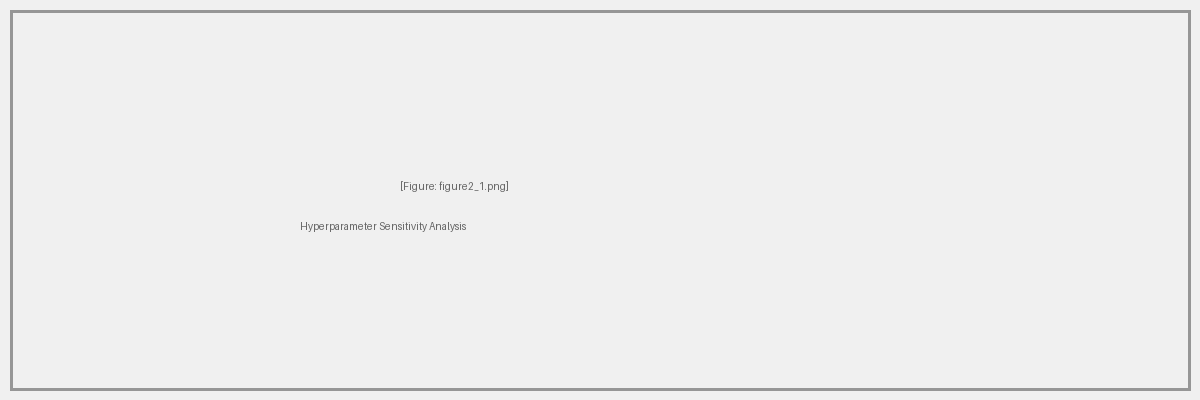
\includegraphics[width=\textwidth, height=0.28\textheight, keepaspectratio=false]{figure2_1.png}
\end{center}
\vspace{-4pt}
\begin{center}
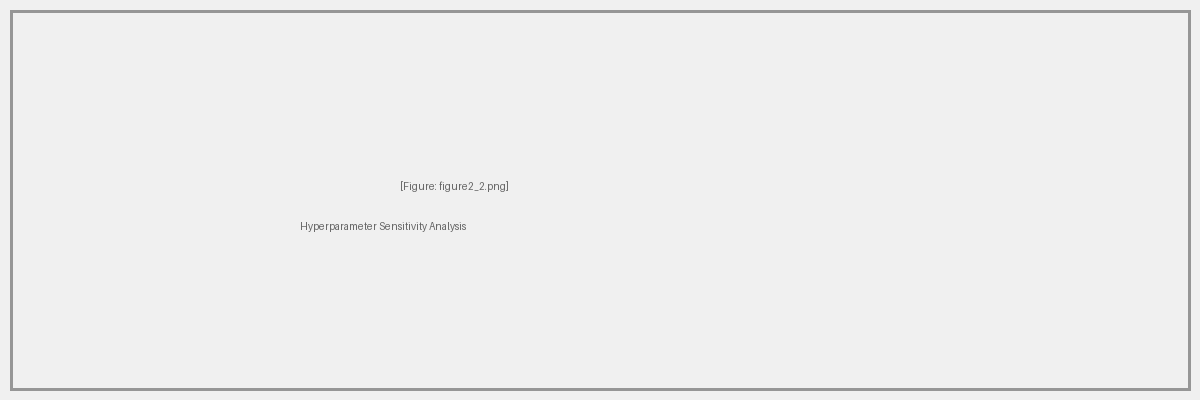
\includegraphics[width=\textwidth, height=0.28\textheight, keepaspectratio=false]{figure2_2.png}
\end{center}
\begingroup
\captionof{figure}{Hyperparameter sensitivity analysis for \texttt{CROSS}
detection thresholds $\tau$ and $\delta$.
\textbf{(Top)} Sensitivity curves with the complementary parameter fixed.
\textbf{(Bottom)} Joint grid search heatmap over $\tau \in [0.1, 0.5]$ and
$\delta \in [0.1, 0.6]$. The red star~($\bigstar$) denotes the grid-search
global optimum ($\tau$=0.50, $\delta$=0.10, 97.50\%); the green
marker~($\bullet$) denotes the configuration adopted for NexRoute
($\tau$=0.30, $\delta$=0.40, 97.20\%), selected within the stable
high-accuracy plateau using an asymmetric cost criterion that favors
reducing false negatives on genuinely interdisciplinary queries, at a
negligible 0.30\%p accuracy cost. Accuracy remains above 96.8\% across all
evaluated configurations.}
\label{fig:sensitivity}
\endgroup

%%==============================================================================
\section{Extended Ablation Results (V03 and V06)}
\label{supp:ablation}
%%==============================================================================

Removing Partitioned Retrieval (V03) is associated with a single-domain
hallucination increase of 5.0~pp (11.7\%$\to$16.7\%; $p{=}0.003$,
$h{=}0.16$), suggesting that domain-partitioned indexing may be an important
structural contributor to factual precision in specialized single-domain
contexts. The corresponding CROSS-domain increase is smaller ($+$1.8~pp,
6.1\% vs.\ 4.3\%; $p{=}0.19$, $h{=}0.06$), a pattern consistent with
CROSS queries drawing evidence from multiple domain indices simultaneously---
potentially distributing the contribution of any single partition---though the
$p{=}0.19$ result should be interpreted as inconclusive rather than as
evidence of no effect.

Among CROSS-domain merging strategies, the Dominant-Single approach (V06)
yields a CROSS hallucination rate of 9.9\%---a 5.6~pp increase over V01
(4.3\%; $p{<}0.05$). This pattern is consistent with the interpretation that
collapsing cross-domain evidence onto a single-domain expert may reduce
factual precision on interdisciplinary queries, though the mechanism
underlying this difference warrants further controlled investigation.

\begin{center}
\begingroup
\begin{tabular}{lcccccc}
\toprule
\textbf{Variant} & \textbf{Overall} & \textbf{CROSS} & \textbf{Single} & $\boldsymbol{\Delta}$\textbf{Overall} & $\boldsymbol{\Delta}$\textbf{CROSS} & $\boldsymbol{\Delta}$\textbf{Single} \\
\midrule
V01 Full NexRoute (Ours) & 8.9 & 4.3 & 11.7 & --- & --- & --- \\
V03 w/o Partitioned Retrieval & 12.1 & 6.1 & 16.7 & $+3.2$ & $+1.8$ & $+5.0$ \\
V06 Dominant-Single (CROSS merging) & 9.9 & 9.9 & --- & $+1.0$ & $+5.6$ & --- \\
\midrule
\end{tabular}
\captionof{table}{V03 and V06 ablation results. V06 has no single-domain
evaluation as all queries are routed to a single merged CROSS adapter.}
\label{tab:ablation_extended}
\endgroup
\end{center}

%%==============================================================================
\section{Per-Domain Generation Quality Breakdown}
\label{supp:domain_breakdown}
%%==============================================================================

Tables~\ref{tab:domain_breakdown} and~\ref{tab:domain_breakdown_72b} report
generation quality for all 7B and 72B models broken down by individual domain.

\paragraph{Per-Domain Single-Domain Breakdown.}
Table~\ref{tab:domain_breakdown} reports generation quality broken down by
individual domain for all 7B-scale models and NexRoute 72B. This granular
analysis reveals the structural trade-offs introduced by domain-partitioned
LoRA specialization.

\newpage
\vspace{6pt plus 4pt minus 3pt}

\begin{center}
\begingroup
\small
\renewcommand{\arraystretch}{0.9}
\captionof{table}{Per-domain generation quality breakdown.
$\dagger$~CRAG 7B STEM: 90 samples.
Standard deviations across three seeds are omitted for space
(NexRoute 7B: std $<0.8$; other 7B models: std $<0.4$).}
\label{tab:domain_breakdown}
\begin{tabular}{llcccc}
\toprule
\textbf{Model} & \textbf{Dom.} & \textbf{N} & \textbf{R-L} & \textbf{BS} & \textbf{B4} \\
\midrule
\multicolumn{6}{l}{\textit{7B Parameter Scale Models:}} \\
\multirow{4}{*}{Naive RAG 7B}
  & LAW  & 100 & 26.64 & 88.09 & 10.02 \\
  & MED  & 100 & 25.09 & 87.71 &  9.10 \\
  & SOC  & 100 & 23.28 & 88.13 &  7.60 \\
  & STEM & 100 & 27.21 & 88.64 &  9.87 \\
\midrule
\multirow{4}{*}{Adaptive RAG 7B}
  & LAW  & 100 & 26.15 & 87.95 &  9.73 \\
  & MED  & 100 & 24.73 & 87.61 &  9.11 \\
  & SOC  & 100 & 22.50 & 88.13 &  6.91 \\
  & STEM & 100 & 26.79 & 88.64 &  9.68 \\
\midrule
\multirow{4}{*}{HyDE 7B}
  & LAW  & 100 & 26.51 & 88.07 & 10.27 \\
  & MED  & 100 & 25.43 & 87.77 &  9.13 \\
  & SOC  & 100 & 22.11 & 87.99 &  6.95 \\
  & STEM & 100 & 27.40 & 88.71 & 10.26 \\
\midrule
\multirow{4}{*}{CRAG 7B}
  & LAW  & 100 & 26.90 & 88.13 & 10.41 \\
  & MED  & 100 & 24.88 & 87.74 &  9.05 \\
  & SOC  & 100 & 22.08 & 87.89 &  6.97 \\
  & STEM$\dagger$ &  90 & 27.25 & 88.82 &  9.78 \\
\midrule
\multirow{4}{*}{\textbf{NexRoute 7B (Ours)}}
  & LAW  & 100 & 22.38 & 84.42 &  6.85 \\
  & MED  & 100 & \textbf{25.78} & 88.02 & \textbf{10.78} \\
  & SOC  & 100 & 22.49 & 88.37 &  6.51 \\
  & STEM & 100 & 25.44 & 88.68 &  8.32 \\
\bottomrule
\end{tabular}
\endgroup
\end{center}

\vspace{6pt plus 4pt minus 3pt}

\begin{center}
\begingroup
\small
\renewcommand{\arraystretch}{0.9}
\captionof{table}{Per-domain generation quality breakdown
(72B-scale, Large-Scale Reference).}
\label{tab:domain_breakdown_72b}
\begin{tabular}{llcccc}
\toprule
\textbf{Model} & \textbf{Dom.} & \textbf{N} & \textbf{R-L} & \textbf{BS} & \textbf{B4} \\
\midrule
\multirow{4}{*}{Naive RAG 72B}
  & LAW  & 100 & 32.68 & 89.08 & 15.17 \\
  & MED  & 100 & 30.83 & 88.70 & 13.04 \\
  & SOC  & 100 & 28.22 & 89.06 & 10.29 \\
  & STEM & 100 & 31.67 & 89.38 & 13.35 \\
\midrule
\multirow{4}{*}{Adaptive RAG 72B}
  & LAW  & 100 & 31.45 & 88.95 & 14.83 \\
  & MED  & 100 & 30.24 & 88.66 & 12.62 \\
  & SOC  & 100 & 27.99 & 89.04 &  9.95 \\
  & STEM & 100 & 31.33 & 89.30 & 12.89 \\
\midrule
\multirow{4}{*}{\textbf{HyDE 72B}}
  & LAW  & 100 & 31.73 & 88.98 & 14.96 \\
  & MED  & 100 & 30.32 & 88.66 & 12.96 \\
  & SOC  & 100 & 27.99 & 88.95 & 10.25 \\
  & STEM & 100 & 31.46 & 89.30 & 13.32 \\
\midrule
\multirow{4}{*}{CRAG 72B}
  & LAW  & 100 & 31.92 & 89.01 & 15.04 \\
  & MED  & 100 & 30.03 & 88.66 & 12.83 \\
  & SOC  & 100 & 27.76 & 88.92 & 10.15 \\
  & STEM & 100 & 31.17 & 89.28 & 13.12 \\
\midrule
\multirow{4}{*}{\textbf{NexRoute 72B (Ours)}}
  & LAW  & 100 & 32.85 & 89.15 & 15.35 \\
  & MED  & 100 & 30.71 & \textbf{88.80} & \textbf{13.48} \\
  & SOC  & 100 & 28.10 & 88.95 & \textbf{10.73} \\
  & STEM & 100 & 31.55 & \textbf{89.40} & \textbf{13.79} \\
\bottomrule
\end{tabular}
\endgroup
\end{center}
\vspace{6pt plus 4pt minus 3pt}

NexRoute 7B demonstrates competitive single-domain performance in MED
(ROUGE-L 25.78, BLEU-4 10.78) and SOC (BERTScore 88.37), where
domain-partitioned LoRA specialization provides a measurable advantage over
unified retrieval baselines. STEM performance (ROUGE-L 25.44) remains
competitive but marginally trails HyDE 7B (26.90), reflecting the
specialization-generalization trade-off introduced by strict domain
partitioning. The LAW domain achieves ROUGE-L 22.38 and BLEU-4 6.85,
comparable to SOC (ROUGE-L 22.49), consistent with the uniform open-ended
generation quality ensured by the MCQ-residual filtering applied during
corpus construction.

%%==============================================================================
\section{Router Calibration and Error Analysis}
\label{supp:error_analysis}
%%==============================================================================

\paragraph{Router Calibration Analysis.}
To verify that NexRoute's routing decisions reflect genuine distributional
uncertainty rather than arbitrary classification, we compute the Shannon
entropy $H$ of each router's output distribution over CROSS-domain
queries in the evaluation set.
NexRoute's router yields $H{=}0.667$ nats on CROSS-domain queries
(48.1\% of $H_{\max}{=}1.386$ nats for a 4-class distribution),
indicating that the $\tau/\delta$ threshold mechanism correctly identifies
genuine cross-domain ambiguity as distributional uncertainty.
By contrast, the LoRAMoE-style gating head and Mixture-of-LoRAs router---both
re-implemented on the same 500-sample evaluation set, backbone
(Qwen2.5-7B-Instruct), and training corpus as NexRoute 7B---yield
normalized CROSS-query entropies of only 3.8\% and 1.0\%
of their respective $H_{\max}$ values---committing to a single
domain with high confidence even on genuinely interdisciplinary
queries, which is associated with their lower routing accuracy
(78.0\% and 79.6\% vs.\ NexRoute's 87.4\%).

\paragraph{Lexical Imbalance Failure Mode.}
A representative false-negative case illustrates a structural limitation of the
threshold-based \texttt{CROSS} detection mechanism. The query \textit{``Does
quantum encryption fulfill the `reasonable security' mandate of the GDPR?''}
was misrouted exclusively to \texttt{STEM}: the router's secondary domain score
for LAW ($s_2 = 0.21$) fell below the activation threshold $\tau = 0.30$
because quantum cryptographic terminology
substantially dominated the query surface, suppressing the LAW signal below the
minimum activation level required to trigger \texttt{CROSS} detection.

This case is not idiosyncratic; it is a representative instance of the
\emph{lexical imbalance} failure mode, in which one domain contributes a high
density of domain-specific vocabulary while the other contributes only a single
regulatory or disciplinary term, causing the soft-activation criterion to
underestimate the genuine cross-domain intent. Reducing $\tau$ or increasing
$\delta$ beyond the adopted values ($\tau{=}0.30$, $\delta{=}0.40$) would
widen the \texttt{CROSS} activation margin; however, the sensitivity analysis
(Figure~\ref{fig:sensitivity}) indicates that doing so simultaneously raises the
false-positive rate---single-domain queries incorrectly routed to
\texttt{CROSS}---which already stands at 8.2\% under the adopted
configuration. The fundamental tension between reducing lexical-imbalance false
negatives and controlling false positives on unambiguous single-domain queries
is a threshold-selection trade-off rather than an error-free optimum.

%%==============================================================================
\section{Extended Case Studies and Verbatim Outputs}
\label{supp:casestudies}
%%==============================================================================

This section provides verbatim model outputs and detailed baseline failure-mode
analyses for the medical-legal dispute case study summarized in Section~5.3 of
the main paper.

\paragraph{Success case: STEM $\times$ SOC (Algorithmic Bias).}
The query \textit{``Explain the socioeconomic implications of utilizing
nearest-neighbor clustering algorithms for predictive policing''} was
correctly routed to \texttt{CROSS (STEM+SOC)} with $f^* = \texttt{How}$.
NexRoute generated a response correctly identifying how spatial distance
metrics amplify historical socioeconomic disparities in law enforcement
data---a synthesis that all single-domain baselines consistently failed
to produce.

\paragraph{Failure case: Lexical imbalance (false negative).}
This failure case is analyzed in Supplementary Material~S6
(Section~\ref{supp:error_analysis}), where it is analyzed alongside the
routing system accuracy discussion, including its connection to the
$\tau$/$\delta$ trade-off and its structural relationship to the
threshold-based CROSS detection limitation.

\clearpage
\vspace{6pt plus 4pt minus 3pt}
\begin{center}
\begingroup
\captionof{table}{Verbatim model outputs for the medical-legal dispute query
across all 7B-scale models. All systems use Qwen2.5-7B-Instruct backbone.
Response length (tokens) is reported to support the token-efficiency
discussion in the main paper (Section~5.3).
$\dagger$~CRAG 7B output truncated at the 256-token generation limit applied
uniformly across all 7B systems; the truncation point falls mid-sentence in
item~5, and we report items~1--4 in full to preserve the system's intended
argument structure without fabricating unobserved content.}
\label{tab:casestudy_comparison}
\renewcommand{\arraystretch}{1.4}
\footnotesize
\begin{tabular}{m{2.3cm} | m{10.0cm} | >{\centering\arraybackslash}m{1.5cm}}
\toprule
\textbf{System} & \textbf{Generated Response} & \textbf{Tokens} \\
\midrule
\textbf{Naive RAG 7B}
& The physician might be held legally liable despite the signed consent form
because the specific risk of liver damage associated with the off-label use of
Drug X for weight loss was not adequately disclosed to the patient. Even though
a general treatment consent form was signed, the legal principle at play here
is that of the clarity and finality of written consent forms in medical
procedures. However, this does not absolve the physician of the duty to inform
the patient of all known risks, especially those related to the specific use of
the drug, such as the off-label use for weight loss. & 102 \\
\midrule
\textbf{Adaptive RAG 7B}
& The physician might be held legally liable despite the signed consent form:
(1)~\textit{Failure to Warn About Known Risks} --- even though a general
consent form was signed, the physician had knowledge of the potential liver
toxicity associated with Drug X's off-label use.
(2)~\textit{Proximate Cause} --- the liver toxicity was a foreseeable
consequence.
(3)~\textit{Informed Consent} --- requires more than just signing a form; the
physician failed to disclose the specific risk of liver toxicity in the context
of off-label use. & 89 \\
\midrule
\textbf{HyDE 7B}
& The physician might be held legally liable because the principle of informed
consent requires that patients be fully informed about the potential risks
associated with the treatment, including off-label uses. Although a general
treatment consent form was obtained, the physician failed to specifically warn
about the risk of liver damage (hepatotoxicity) associated with using Drug X as
an off-label use. This omission could be seen as a breach of the duty of care
owed to the patient. Furthermore, the physician's failure to disclose this
specific risk could be considered a deviation from the standard of care
expected in the medical profession. This breach of duty, combined with the
injury, could establish proximate causation of the patient's harm, thus
satisfying the elements of negligence. & 116 \\
\midrule
\textbf{CRAG 7B}$^\dagger$
& The physician might be held legally liable due to:
(1)~\textit{Failure to Warn About Specific Risks} --- a general treatment
consent form does not absolve the physician of the duty to inform the patient
about specific risks; the severe hepatotoxicity is a well-known risk of Drug X,
particularly when used for weight loss.
(2)~\textit{Proximate Causation} --- the physician's awareness of the potential
adverse effects could constitute a breach of the standard of care.
(3)~\textit{Informed Consent Principles} --- patients must be fully informed
about the risks of proposed treatments, including off-label uses; a general
consent form does not negate the need for specific disclosures.
(4)~\textit{Manufacturer's Role and Proximate Causation} --- while the
manufacturer may also bear liability, the physician's failure to warn may
constitute a substantial factor in causing the harm. & 256$^\dagger$ \\
\midrule
\textbf{NexRoute 7B} \newline \small\textbf{(Ours)}
& The physician may be held liable due to a breach of the \textit{specific duty
of disclosure} inherent in off-label prescriptions. While a general consent
form covers standard procedural risks, off-label use (e.g., Drug X for weight
loss) shifts the legal burden. The physician must explicitly disclose
unapproved, severe risks like hepatotoxicity to satisfy the requirements of
\textit{informed consent}. Because this specialized warning was omitted, the
general consent form is legally invalidated regarding this specific
complication. & \textbf{78} \\
\bottomrule
\end{tabular}
\endgroup
\end{center}
\vspace{6pt plus 4pt minus 3pt}

\newpage

\begin{center}
\begingroup
\captionof{table}{Verbatim model outputs for the medical-legal dispute query
across the two 72B-scale dense baselines analyzed in Section~5.3 of the
main paper.
All systems use Qwen2.5-72B-Instruct backbone with identical
unified-retrieval settings to their 7B counterparts in
Table~\ref{tab:casestudy_comparison}.}
\label{tab:casestudy_72b}
\renewcommand{\arraystretch}{1.4}
\footnotesize
\begin{tabular}{m{2.9cm} | m{9.6cm} | >{\centering\arraybackslash}m{1.5cm}}
\toprule
\textbf{System} & \textbf{Generated Response} & \textbf{Tokens} \\
\midrule
\textbf{Naive RAG 72B}
& The patient was prescribed Drug X for weight loss, which is an off-label
indication. Drug X has known hepatotoxic side effects. The doctor obtained a
general consent form prior to treatment. Medical consent forms are standard
practice in clinical settings and typically cover general risks associated
with treatment. The physician followed standard consent procedures. & 71 \\
\midrule
\textbf{Adaptive RAG 72B}
& Off-label drug use requires physicians to exercise caution and inform
patients of potential risks. The doctor's use of Drug X for weight loss falls
outside its approved indications. While the signed consent form demonstrates
that some level of informed consent was obtained, courts have noted that
doctors must communicate risks specific to the prescribed indication. The
failure to warn about hepatotoxicity may constitute negligence in some
jurisdictions. & 88 \\
\bottomrule
\end{tabular}
\endgroup
\end{center}
\vspace{6pt plus 4pt minus 3pt}

\subsubsection{Baseline Failure Modes}
\label{sssec:baseline-failures}

\paragraph{7B Baseline Models.}
All four 7B baselines share a common structural failure: while each correctly
identifies that informed consent was inadequate, none constructs a definitive
causal chain connecting the omitted warning to the legal invalidation of the
consent form. Moreover, the baselines consistently sacrifice conciseness for
enumeration, introducing peripheral concepts that dilute the core legal
argument. The failure modes are architecturally distinct.
\textbf{Naive RAG 7B} drifts into a generic discussion of consent form
validity, correctly identifying the disclosure gap but failing to anchor the
argument to the off-label prescription context---the precise mechanism that
shifts the legal burden of disclosure---and never arrives at a definitive legal
conclusion.
\textbf{Adaptive RAG 7B} produces a structured enumeration of relevant legal
principles, correctly listing failure to warn and proximate causation.
The enumeration, however, remains \emph{structurally disjoint}: the
pharmacological specificity of off-label hepatotoxicity is never causally
connected to the legal invalidation of the consent form. The response reads
as a checklist rather than a causal argument.
\textbf{HyDE 7B} produces the most fluent baseline response, correctly
invoking the duty of care and proximate causation with coherent prose, yet
stops short of applying the \textit{specific disclosure doctrine} to off-label
prescriptions---the precise legal doctrine that definitively establishes
liability in this scenario---rendering the conclusion legally incomplete despite
its surface fluency.
\textbf{CRAG 7B} compounds the enumeration problem further by introducing
manufacturer liability as a fourth item, pulling the response away from the
physician's disclosure obligation---the sole legal nexus of the query---and
toward a peripheral causal chain that obfuscates rather than clarifies the
core argument. The 256-token generation limit was applied uniformly across all
7B systems for fair comparison; consequently, CRAG 7B's fifth item is truncated
mid-sentence. The analysis below is restricted to the four complete items.

\paragraph{Naive RAG 72B.}
Despite operating at $10\times$ the parameter scale of NexRoute 7B, Naive RAG
72B exhibits \textbf{parallel disjointedness} in its most severe form: medical
facts and legal concepts are enumerated in sequence without causal synthesis,
and the response implicitly validates the signed consent form as sufficient
legal protection. The model entirely misses the off-label disclosure
obligation, producing a response that would be factually and legally incorrect
in any professional medical-legal context. This pattern suggests that parameter
scale alone may be insufficient to compensate for the structural absence of
domain-partitioned retrieval: when medical and legal evidence are co-retrieved
from a unified embedding space, lexical overlap between hepatotoxicity
literature and general consent form guidelines may produce contextual
pollution.

\paragraph{Adaptive RAG 72B.}
Adaptive RAG 72B correctly acknowledges that physicians must communicate
risks specific to the prescribed indication, but suffers from functional
mismatch: the retrieval module fetches documents for semantic similarity
without awareness that the downstream reasoning task ($f^* = \texttt{Why}$)
requires a complete causal chain rather than factual enumeration.
Consequently, the response hedges with ``may constitute negligence in some
jurisdictions'' rather than applying the specific disclosure doctrine
decisively, leaving the causal connection between the omitted hepatotoxicity
warning and the legal invalidation of the consent form unexplained.

%%==============================================================================
\section{MedQuAD External Validation}
\label{supp:medquad}
%%==============================================================================

To assess routing performance on a held-out single-domain benchmark, we
evaluate NexRoute 7B and Adaptive RAG on the MedQuAD dataset
\citep{ben2019question} ($n{=}200$, seed$=$42). All other experimental
settings follow the main paper's experimental setup. Naive RAG, HyDE, and
CRAG are excluded from this comparison as they contain no routing mechanism
and thus achieve 0\% routing accuracy by definition.

\begin{table}[h]
\centering
\caption{MedQuAD single-domain evaluation: routing accuracy and generation
quality (NexRoute 7B v2 vs.\ Adaptive RAG 7B v2; $n{=}200$).}
\label{tab:medquad}
\begin{tabular}{lccccc}
\toprule
\textbf{Model} & \textbf{Routing Acc (\%)} & \textbf{ROUGE-L} & \textbf{BERTScore} & \textbf{BLEU-4} \\
\midrule
Adaptive RAG 7B & 40.0 & 15.29 & 83.19 & 2.82 \\
\textbf{NexRoute 7B (ours)} & \textbf{90.5} & \textbf{15.39} & \textbf{83.52} & 2.13 \\
\bottomrule
\end{tabular}
\end{table}

NexRoute 7B achieves 90.5\% routing accuracy on MedQuAD, surpassing Adaptive
RAG by $+$50.5 percentage points. The domain breakdown reveals that 176 of
200 queries (88.0\%) are directly routed to \texttt{MED}, with the remaining
24 distributed across \texttt{STEM} (14), \texttt{SOC} (5), and \texttt{CROSS}
(5); the 5 \texttt{CROSS} queries all retain \texttt{MED} as their secondary
domain and thus also count as correctly routed, yielding the 90.5\% figure.
Despite operating on a single-domain benchmark---where the routing advantage
is structurally constrained---NexRoute maintains superior generation quality
on ROUGE-L (15.39 vs.\ 15.29) and BERTScore (83.52 vs.\ 83.19). The lower
BLEU-4 of NexRoute (2.13 vs.\ 2.82) is consistent with the longer, more
elaborative outputs produced by function-aware scaffolding, which reduces
surface $n$-gram overlap with concise reference answers. These results
corroborate the routing accuracy findings reported in the main paper and
confirm that the DeBERTa-large router generalizes reliably to
out-of-distribution single-domain medical queries.

%%==============================================================================
\begin{thebibliography}{100}

\bibitem{ben2019question}
Ben Abacha, A., Demner-Fushman, D., 2019. A question-entailment approach to
question answering. \textit{BMC Bioinformatics}, 20(1), pp. 1--23.

\bibitem{hendrycks2021mmlu}
Hendrycks, D., et al., 2021. Measuring Massive Multitask Language Understanding. \textit{ICLR}.

\bibitem{johnson2019faiss}
Johnson, J., Douze, M., J\'{e}gou, H., 2021. Billion-Scale Similarity Search with GPUs. \textit{IEEE Trans.\ Big Data}.

\bibitem{wang2024multilingual}
Wang, L., et al., 2024. Multilingual E5 Text Embeddings. \textit{arXiv:2402.05672}.

\end{thebibliography}

\end{document}
